\documentclass{article}
\usepackage[utf8]{inputenc}
\usepackage{amsmath}
\usepackage{amsfonts}
\usepackage{graphicx}
\usepackage{multicol}
\usepackage{float}
\usepackage{cite}
\usepackage{url}
\usepackage{listings}
\usepackage{pythonhighlight}

\begin{document}
	\begin{titlepage}
		\begin{center}
			{\huge\textbf{Instituto Politécnico Nacional}}\\
			\vspace{7mm}
			{\huge\textbf{Escuela Superior de Cómputo}}\\			
			\begin{figure}[h]
				\centering
				
\includegraphics[height = 6cm]{logoEscom.png}
			\end{figure}	
			\vspace{1cm}
			{\huge\textbf{Programa 6: Autómata de Pila}}
			\par\vspace{2cm}
			\large\textbf{Autor: Colín Ramiro Joel}
			\par\vspace{1cm}
			{\large\textbf{Materia: Teoría de la Computación}}
			\par\vspace{1cm}
			{\large\textbf{Grupo: 4CM2}}
			\par\vspace{1cm}
			{\large\textbf{Profesor: Juarez Martínez Genaro}}
			\par\vspace{1cm}
			{\large\textbf{Fecha de entrega: {\huge{29 de Diciembre 2021}}}}
			\par\vspace{3cm}
		\end{center}
	\end{titlepage}
	\section*{Introducción}
	Un autómata de pila es un modelo matemático el cual en forma similar a como se usan los autómatas finitos, también se puede utilizar para aceptar cadenas de un lenguaje definido sobre un alfabeto en concreto.
	Este lenguaje que reconoce el autómata, pertenece al grupo de los lenguajes libres de contexto en la clasificación de la \textbf{Jerarquía de Chomsky.}
	Estos autómatas pueden aceptar lenguajes que no pueden aceptar los autómatas finitos. Cuenta con una cinta de entrada y un mecanismo de control que puede encontrarse en uno de entre un número finito de estados. Uno de estos estados se designa como
	\textbf{estado inicial}, a su vez cuenta con estados llamados de aceptación o finales. 
	A diferencia de los	autómatas finitos, los autómatas de pila cuentan con una memoria auxiliar llamada pila. Estos símbolos anteriormente mencionados, pueden ser insertados(push) o extraídos(pop) de la pila, de acuerdo con el manejo Last-Input-First-Output (LIFO).
	Las transiciones entre los estados que ejecutan los autómatas de pila dependen de los símbolos de entrada y de los símbolos de la pila. El autómata acepta una cadena \text{X} si la secuencia de transiciones,
	comenzando en estado inicial y con pila vacía, conduce a un estado final, después de leer toda la	cadena \text{X}. 

	Formalmente, el autómata de pila puede definirse como una séptupla tal que: APD=(E,$\Sigma$ ,$\Gamma$ ,$\delta$ ,q0,Z,F) donde:
	
	\begin{itemize}
		\item E = Conjunto finito de estados.
		\item $\Sigma$ = Alfabeto o conjunto finito de símbolos de la cinta de entrada.
		\item $\Gamma$ = Alfabeto o conjunto finito de símbolos de la pila.
		\item $\Delta$ = Función de transición de estados.
		\item q0 = Estado Inicial. 
		\item Z = Símbolo distinguido.
		\item F =Conjunto de estados finales o de acpetación.
		
	


	\end{itemize}
	
	
	
	
	

	\section*{Instrucciones}
	Programar un autómata de pila que sirva para reconocer el lenguaje libre de contexto:\[{{0^{n} 1^{n} | n \geq 1}}\]
	Adicionalmente, el programa debe de contar con las siguientes características:	
	\begin{enumerate}
		\item La cadena puede ser ingresada por el usuario o automáticamente. Si es aleatoriamente, la cadena no podrá ser mayor a \textbf{100,000} caracteres.
		\item Mandar a un archivo y en pantalla la evaluación del autómata a través de descripciones instantáneas(IDs).
		\item Animar el autómata de pila, solo si la cadena es menor o igual a 10 caracteres.
		\item En el reporte debe de estar también el código de implementación en latex, no en imágenes.		
	\end{enumerate}
	\section*{Desarrollo}
	Este programa se realizó mediante el lenguaje de programación \textbf{Python}, esto debido a que para la implementación de la pila no es necesario definir una estructura extra, como lo pueden ser los nodos en otros lenguajes, sino que se pueden utilizar las mismas listas para su utilización. 
	
	El programa se realizó con el mismo formato que otros de los mismos revisados previamente en el curso, con esto me refiero a que cuentan con un menú principal, el cual, le preguntará al usuario si desea introducir la cadena a la que se le aplicará la evaluación o bien que esta se genere automáticamente. En el caso de que el usuario seleccione el modo "manual", el programa le solicitará al usuario que introduzca la cadena deseada. 
	
	Posteriormente se implementaron 2 funciones las cuales realizarán un 90 Por ciento del programa. 
	La primer función es llamada \textbf{evaluarCadena}, lo que realiza esta función básicamente es como bien su nombre lo dice, evalua la cadena definida por el usuario o generada, para identificar si pertenece al lenguaje libre de contexto previamente definido en la sección de \textbf{Instrucciones}. Y la segunda función realiza lo que viene siendo la animación de la pila, esto fue logrado gracias a la libreria \textbf{tkinter}.
	Para terminar con esta sección cabe mencionar que el programa genera un archivo de texto llamado \textbf{SalidaP6.txt} en el cual se encuentran  las Descripciones Instantáneas(ID's) de cada paso que se llevo a cabo para la evaluación de la cadena. 
	
	\section*{Capturas del Funcionamiento}
	Como bien se ha mencionado en reportes pasados, en esta sección se encuentran lo que son las capturas del funcionamiento del programa. Para  una mejor visualización estan separados considerando si es manual o automática la definición de la cadena:
	\begin{enumerate}
		\item \textbf{Cadena Manual}
		\begin{itemize}
			\item 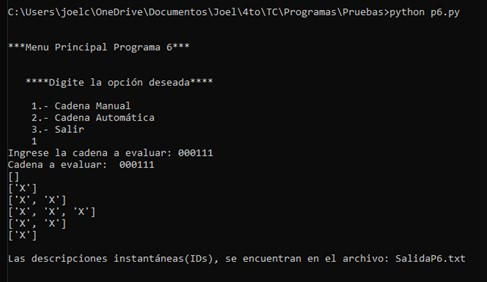
\includegraphics[height = 4cm]{CM5.jpg}
			\item 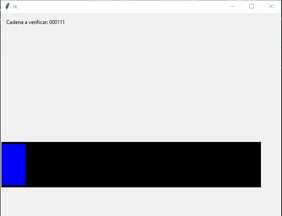
\includegraphics[height = 4cm]{CM1.jpg}
			\item 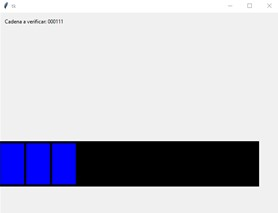
\includegraphics[height = 4cm]{CM3.jpg}
			\item 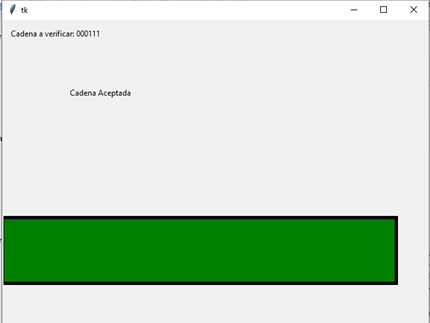
\includegraphics[height = 4cm]{CM4.jpg}
			\item 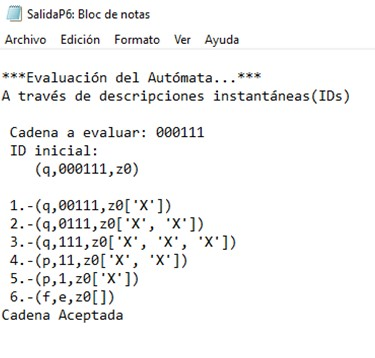
\includegraphics[height = 4cm]{CM6.jpg}
		\end{itemize}		
		\item \textbf{Cadena Automática}
		\begin{itemize}
			\item 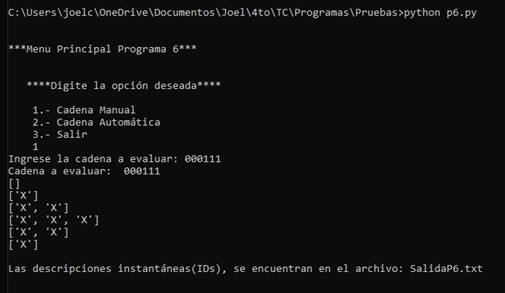
\includegraphics[height = 4cm]{CA3.jpg}
			\item 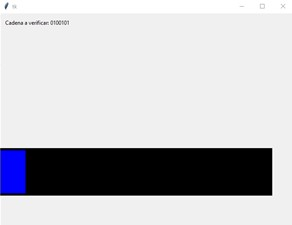
\includegraphics[height = 4cm]{CA1.jpg}
			\item 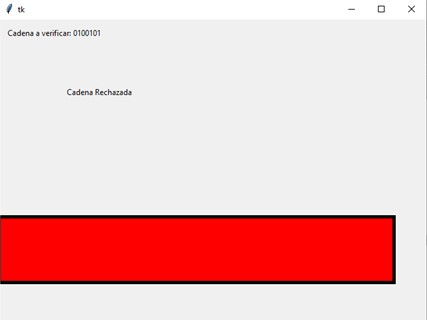
\includegraphics[height = 4cm]{CA2.jpg}
			\item 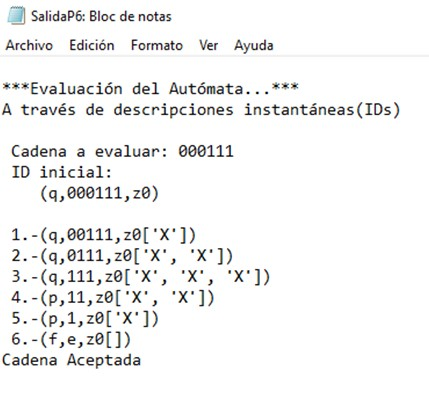
\includegraphics[height = 4cm]{CA4.jpg}
		\end{itemize}		
		
	\end{enumerate}
	
	\section*{Código}
	\begin{python}
		# Programa 6.Autómata de Pila
		# Nombre: Colín Ramiro Joel
		# Profesor: Juarez Martínez Genaro
		# Grupo: 4CM2
		# Materia: Teoría Computacional
		import time
		import random
		from tkinter import*
		
		def animarPila(cad):        
			ventana = Tk()
			ca = Canvas(ventana, width=650, height=650) 
			ventana.geometry("650x650")
			ca.place(x=0,y=0)
			et = Label(ventana, text = "Cadena a verificar: " + cad).place(x=10,y=10)
			ca.create_rectangle(0,300, 600, 400, width=5, fill='black')    
			xIni = 0
			xFin = 60
			yIni = 300
			yFin = 400
			cadList = list(cad)
			lenCadList = len(cadList)
			cadList.append("")
			for caracter in cadList:        
				ventana.update()
				time.sleep(.5)        
				if(caracter == "0"):
					ca.create_rectangle(xIni, yIni, xFin, yFin, width=5, fill='blue')
					xIni = xIni + 60
					xFin = xFin + 60 
					lenCadList = lenCadList - 1 
					if(lenCadList == 0):
						cadEtiqueta = Label(ventana, text="Cadena Rechazada \n").place(x=100,y=100)  
						ca.create_rectangle(0,300, 600, 400, width=5, fill='red')
					break 
				elif(caracter == "1"):
					ca.create_rectangle(xIni-60, yIni, xFin-60, yFin, width=5, fill='black')
					xIni = xIni - 60
					xFin = xFin - 60
					lenCadList = lenCadList - 1 
					if(lenCadList == 0):
						cadEtiqueta = Label(ventana, text="Cadena Rechazada \n").place(x=100,y=100)  
						ca.create_rectangle(0,300, 600, 400, width=5, fill='red')
					break
				elif(caracter == ""):
					ca.create_rectangle(0,300, 600, 400, width=5, fill='green')
					cadEtiqueta = Label(ventana, text="Cadena Aceptada\n").place(x=100,y=100)
					break
				lenCadList = lenCadList - 1
			ventana.mainloop()
		
		def evaluarCadena(opcion):
			archivo = open("SalidaP6.txt","w")
			archivo.write("\n***Evaluación del Autómata...***\n")
			archivo.write("A través de descripciones instantáneas(IDs)")
			if(opcion == 1):
				cadena = input("Ingrese la cadena a evaluar: ")
				cad = list(cadena)
				cad.append("")
			elif( opcion == 2):
				rand = random.randrange(100000)
				cadena = str(bin(rand)[3:])
				cad = list(cadena)     
				cad.append("")   
				print("Generando cadena...")
			print("Cadena a evaluar: ", cadena)
			archivo.write("\n\n Cadena a evaluar: " + cadena + "\n")
			longCad = len(cad)
			if(longCad <= 10):
				animarPila(cadena)
			pila = []
			print(pila)    
			estado = "q"    
			archivo.write(" ID inicial: \n")  
			archivo.write("    (" + estado + "," + cadena + "," + "z0" + ")\n")   
			for caracter in range(0,longCad):    
				archivo.write("\n " + str(caracter+1) + ".-")       
				time.sleep(.5)   
				if(len(pila) == 0):
					estado = "f"                                  
					if(cad[caracter] == "1"):
						estado = "p"
						archivo.write("(" + estado + "," + cadena[caracter:longCad] + "," + "z0" + ")")   
						print("Cadena Rechazada")
						archivo.write("\nCadena Rechazada") 
						break                
					elif(cad[caracter] == "0"):
						estado = "q"
						time.sleep(.5)
						pila.append("X")
						archivo.write("(" + estado + "," + cadena[caracter+1:longCad] + "," + "z0" + str(pila) + ")")   
					else:
						archivo.write("(" + estado + "," + "e" + "," + "z0" + ")")   
						print("Cadena Aceptada")          
						archivo.write("\nCadena Aceptada")                
				else:
					if(cad[caracter] == ""):
						estado = "f"                                  
						archivo.write("(" + estado + "," + "e"+ "," + "z0" + ")")   
						print("Cadena Rechazada") 
						archivo.write("\nCadena Rechazada")    
						break
					elif(cad[caracter] == "1"):
						time.sleep(.5)
						pila.pop() 
						if(cad[caracter+1] == ""):
							estado = "f"
							archivo.write("(" + estado + "," + "e" + "," + "z0" + str(pila) + ")")    
							archivo.write("\nCadena Aceptada")             
							break
						else:
							estado = "p"                       
							archivo.write("(" + estado + "," + cadena[caracter+1:longCad] + "," + "z0" + str(pila) + ")")        
					elif(cad[caracter] == "0"):
						estado = "q"
						time.sleep(.5)
						pila.append("X")
						archivo.write("(" + estado + "," + cadena[caracter+1:longCad] + "," + "z0" + str(pila) + ")")             
				print(pila)
			print("\nLas descripciones instantáneas(IDs), se encuentran en el archivo: SalidaP6.txt")
		
		opc = 0
		salir = 3
		while opc != salir:
			print("\n\n***Menu Principal Programa 6***\n\n")
			print("   ****Digite la opción deseada****")
			opc = int(input('''
			1.- Cadena Manual
			2.- Cadena Automática
			3.- Salir
			'''))    
			if (opc == 1) or (opc == 2):
				evaluarCadena(opc)    
			elif opc == 3:
				print("Saliendo del Programa. Hasta Luego!!!!")
			else:
				print("Opcion inválida, Vuelva a intentar")

	\end{python}
	
	\section*{Conclusiones}
	Para este 6to programa puedo concluir que fue algo sencillo la implementación de la pila, ya que lo realice mediante el lenguaje de programación Python, en el cual no es del todo necesario prescindir de una estructura como pueden ser los nodos en C++ para la implementación de esta estructura de datos. Se recurrió a la utilización de listas, como se mencionó en la sección del Desarrollo. 
	
	Lo que resultó un poco complejo de implementar más que nada fue la parte de la animación de la pila ya que como se puede observar, decidí separar las funciones. Sin embargo, recurrí a varias fuentes bibliográficaas asi como video tutoriales para su elaboración. 
	Lo que puedo concluir con respecto al programa es que es bastante interesante todo el proceso que existe dentro de la teória de autómatas con respecto a las pilas. Cuando originalmente me fue enseñado este tema en las clases de programación, no me imaginaba todo el alcance que estas estructuras de datos pueden tener y el futuro que les espera.
	
	\section*{Referencias}
	\begin{enumerate}
		\item UNICEN. (2008). Autómata de Pila. Diciembre 21,2021, de UNICEN Sitio web: https://users.exa.unicen.edu.ar/catedras/ccomp1/Apunte4.pdf
		
		\item INAOE. (2014). Autómatas de Pila. Diciembre 21, 2021, de INAOE Sitio web:  https://ccc.inaoep.mx/~emorales/Cursos/Automatas/AutomatasPila.pdf
		
		\item BUAP. (2018). Unidad 4. Autómatas de Pila. Diciembre 21,2021, de BUAP Sitio web: https://www.cs.buap.mx/~mtovar/doc/LFAA/Unidad4AP.pdf
	\end{enumerate}
	
\end{document}